\subsection{Bases de datos}
\label{subsection:Database}

Para integrar las condiciones ambientales que caracterizan el periodo comprendido entre la siembra y la emergencia del maíz, en este trabajo se emplean las bases de datos ráster desarrolladas por el Servicio Meteorológico Alemán (DWD, por sus siglas en alemán). Estas bases de datos son generadas mediante técnicas y modelos de interpolación previamente establecidos y se encuentran sujetas a procesos continuos de mantenimiento y control de calidad por parte del DWD.\\

Al contar con cobertura nacional de Alemania, alta resolución espacial, consistencia metodológica, amplia disponibilidad de datos históricos y soporte institucional, estas bases de datos constituyen fuentes de información confiables para la incorporación de registros agroclimáticos y favorecen la reproducibilidad de los resultados.\\

\subsubsection{HYRAS}

El repositorio Hydrometeorologische Rasterdatensätze (HYRAS), versión v6-1, alberga las bases de datos históricos referentes a la temperatura ambiente \citep{DWD_HYRAS_MaxTemp, DWD_HYRAS_MeanTemp, DWD_HYRAS_MinTemp} y la humedad relativa \cite{DWD_HYRAS_RelHumidity} a nivel nacional. Empleando los registros diarios, desde 1951 a la fecha, medidos a través de 1300 estaciones climáticas distribuidas en Alemania y sus siete países vecinos \citep{Razafimaharo_2020}, se genera un archivo ráster por día, con una resolución espacial de $1\times1$ km, a partir de la metodología de interpolación propuesta por \cite{Krhenmann_2016}\\



Las bases de datos en HYRAS han sido sometidas a una extensa validación. A distintas escalas temporales (día, mes, año y el periodo completo de observación), se han comparado las mediciones registradas en las estaciones con los valores interpolados correspondientes a la celda más cercana así como a lo largo de los distintos niveles de elevación del terreno \citep{Razafimaharo_2020}. Asimismo, de acuerdo con \cite{Razafimaharo_2020}, las bases de datos de este repositorio han sido comparadas con bases de datos homólogas, como el Gridded European Climate Assessment y el conjunto de datos mensuales del DWD.\\

Estas evaluaciones han demostrado una alta fidelidad entre las bases de datos del repositorio HYRAS y las correspondientes observaciones \textit{in situ}. Sin embargo, la precisión de la interpolación puede disminuir en regiones con topografía compleja, particularmente para la humedad relativa, mientras que para la temperatura conserva datos altamente comparables \citep{Razafimaharo_2020}.\\

Del repositorio HYRAS, se emplean las bases de datos de temperatura media \citep{DWD_HYRAS_MeanTemp} y humedad relativa \citep{DWD_HYRAS_RelHumidity} a lo largo de este trabajo al ser variables ambientales que participan durante el periodo fenológico comprendido entre la siembra y la emergencia del maíz.\\

Además, las características como el formato ráster, la rigurosidad metodológica, el control de calidad en los datos y la resolución espacial, permiten una representación homogénea de las condiciones ambientales en el espacio y el tiempo que resulta adecuada para análisis agrícolas a escala regional al reducir las inconsistencias asociadas con los registros de estaciones individuales.\\

\subsubsection{Ráster diarios de la temperatura del suelo a una profundidad de 5 cm}

El modelo AMBETI es una herramienta multipropósito diseñada para simular las interacciones suelo-planta-atmósfera, incluyendo el transporte de vapor de agua y agua líquida a través del suelo, así como los flujos netos de radiación en las superficies de la planta y del suelo \citep{Braden_1995}. Específicamente, la componente de termodinámica del suelo es utilizado por el DWD para estimar la temperatura diaria del suelo a una profundidad de 5 cm desde 1991, dando lugar a este conjunto de datos.\\


A partir de la interpolación de mediciones \textit{in situ} provenientes de aproximadamente 280 estaciones distribuidas en Alemania, se generan archivos ráster ASCII diarios con resolución de $1\times1$ km. La temperatura del suelo se estima inicialmente en las estaciones meteorológicas mediante el modelo AMBETI y posteriormente se interpola mediante una regresión lineal múltiple regional basada en la longitud, latitud y elevación, seguida de una triangulación para generar datos espaciales continuos sobre Alemania \citep{DWD_soiltemperature}.\\

De acuerdo con \cite{DWD_soiltemperature}, las interpolaciones resultantes son físicamente factibles dado que la temperatura del suelo está determinada principalmente por la temperatura atmosférica y la radiación solar incidente, como señalan \cite{BAUMBERGER_2024}. En consecuencia, la temperatura del suelo tiende a presentar una baja variabilidad \citep{DWD_soiltemperature}.\\ 


Lo anterior sustenta la validez metodológica de la interpolación en conjuntos de datos en formato de ráster \citep{Schloeder_2001}. Por lo tanto, el procedimiento de interpolación proporciona estimaciones espaciales confiables en Alemania, siendo la principal fuente de incertidumbre durante el invierno la distribución espacial heterogénea de la cobertura de nieve \citep{DWD_soiltemperature}.\\

Para el desarrollo de este trabajo, se seleccionó esta base de datos debido a que representa de manera cercana el ambiente térmico experimentado por las semillas de maíz durante el periodo comprendido entre la siembra y la emergencia. Asimismo, su disponibilidad diaria, cobertura nacional, resolución espacial y metodología de estimación basada en principios físicos robustece la representación de las condiciones ambientales que influyen en el periodo de siembra a emergencia de la secuencia fenológica.\\

\subsubsection{Ráster diarios de la humedad del suelo para el maíz en Alemania}

La base de datos de humedad del suelo para el cultivo de maíz fue generado mediante el modelo Agrarmeteorologische Berechnung der Aktuellen Verdunstung (AMBAV) 2.0, versión 1.5, un modelo agrohidrológico basado en principios físicos que simula la dinámica del agua en el suelo dentro del sistema suelo-planta \citep{DWD_soilmoisture_maize}. Como describen \cite{Herbst_2021}, se modela el almacenamiento de agua en el suelo considerando el consumo hídrico del cultivo, obteniendo una caracterización específica de la dinámica de la humedad del suelo para cada cultivo.\\

Las mediciones \textit{in situ}s de variables meteorológicas, incluyendo la temperatura del aire, humedad relativa, radiación de onda corta y onda larga, precipitación y velocidad del viento, obtenidas de las estaciones del DWD cada hora, se utilizan para la interpolación espacial y la posterior estimación de la disponibilidad de agua en el suelo \citep{Herbst_2021}.\\

El balance hídrico del suelo se parametriza mediante perfiles específicos para cada cultivo, que incorporan factores como la demanda hídrica del cultivo, el desarrollo radicular y la dinámica de extracción de agua, permitiendo derivar el contenido de agua disponible para las plantas en cada cultivo \citep{Herbst_2021}; en este caso, el maíz.\\

A partir de 1991, el conjunto de datos resultante proporciona archivos ráster diarios que cubren Alemania con una resolución espacial de $1 \times 1$ km, los cuales contienen estimaciones de humedad del suelo específicas para cada cultivo, expresadas como porcentaje de la Capacidad de Campo Disponible (AFC, por sus siglas en inglés) \citep{DWD_soilmoisture_maize}, que indica la proporción de agua disponible para las plantas en el suelo \citep{DWD_nFK}.\\

La base de datos contiene perfiles verticales del agua en el suelo mediante capas de 10 cm de espesor desde la superficie hasta una profundidad de 2 m, además de capas agregadas que representan la disponibilidad acumulada de agua dentro de los perfiles de suelo de 0-30, 0-60 y 0-90 cm \citep{DWD_soilmoisture_maize}.\\

Para este trabajo, se seleccionó la capa de humedad del suelo de 0-10 cm, la zona del suelo donde se deposita la semilla de maíz, inicia la imbibición y ocurre el desarrollo radicular temprano. Considerando la cobertura territorial, resolución espacial, disponibilidad de datos y metodología de interpolación, esta base de datos proporciona una representación confiable de la disponibilidad de agua en el suelo durante las primeras etapas del cultivo, consolidando el conjunto de las condiciones ambientales que influyen en el periodo comprendido entre la siembra y la emergencia del maíz.\\

\subsubsection{Datos ambientales}

De las variables disponibles en los bases de datos del DWD descritos anteriormente, se seleccionó un subconjunto de acuerdo con sus interacciones durante el periodo comprendido entre la siembra y la emergencia del maíz, considerando los requerimientos meteorológicos, hídricos y térmicos. Aunque las extensiones temporales de los conjuntos de datos se remontan a fechas anteriores a 1996, en este estudio únicamente se consideró el periodo común comprendido entre 1996 y 2025. Las variables extraídas de cada conjunto de datos, junto con sus respectivas características, se resumen en la Tabla \ref{table:Vars}.\\



\begin{table}[ht]
	\small
	\centering
	\begin{tabular}{>{\raggedright\arraybackslash}p{4cm}
			|>{\centering\arraybackslash}p{1.8cm}
			|>{\raggedright\arraybackslash}p{4.7cm}
			|>{\centering\arraybackslash}p{2.0cm}
			|>{\centering\arraybackslash}p{2.1cm}}
		\hline
		\textbf{Variable ambiental} &
		\textbf{Unidad de medida} &
		\textbf{Base de datos} &
		\textbf{Frecuencia de registro} &
		\textbf{Periodo de estudio} \\ \hline
		
		Temperatura ambiental media &
		$^\circ$C &
		\multirow{2}{=}{HYRAS} &
		\multirow{7}{=}{Diaria} &
		\multirow{7}{=}{1996--2025} \\ \cline{1-2}
		
		
		Humedad relativa ambiental media &
		\% &
		&
		&
		\\ \cline{1-3}
		
		Temperatura media en el suelo (5 cm profundidad)*&
		$^\circ$C &
		Ráster diarios de la temperatura del suelo a una profundidad de 5 cm &
		&
		\\ \cline{1-3}
		
		Humedad media en el suelo (0--10 cm profundidad) &
		\% AFC &
		Ráster diarios de la humedad del suelo para el maíz en Alemania &
		&
		\\ \hline
		
	\end{tabular}
	\caption{Variables ambientales utilizadas en este trabajo, incluyendo sus unidades de medida, bases de datos de procedencia, frecuencia de registro y periodo de estudio. *Los valores originales deben dividirse entre diez para obtener la unidad correcta de $^\circ$C \citep{DWD_soiltemperature}.}
	\label{table:Vars}
\end{table}


\subsubsection{Requerimientos ambientales}
El periodo de la secuencia fenológica del maíz que comprende desde la siembra de la semilla hasta la emergencia de la plántula, cuando se desarrolla exitosamente, tiene una duración de  $16.6 \pm 3.1$ días \citep{CHMIELEWSKI_2004}.  Durante esta etapa, el cultivo es altamente susceptible a las condiciones del entorno \citep{Sanchez_2013}, motivo por el cual los requerimientos ambientales han sido descritos en la literatura previa.\\

Considerando los datos ráster disponibles descritos previamente (ver Tabla \ref{table:Vars}) y tras una revisión bibliográfica, se recopilaron los valores y rangos de condiciones ambientales sugeridos como favorables para el desarrollo de la semilla y la emergencia de la plántula. Estos valores se emplearon como referencia para establecer las condiciones ambientales evaluadas en el modelo y se resumen en la Tabla \ref{tab:optimal_conditions}.\\

\begin{table}[ht]
	\small
	\centering
	\begin{tabular}{>{\raggedright\arraybackslash}p{3.5cm}
			|>{\raggedright\arraybackslash}p{4.5cm}
			|>{\centering\arraybackslash}p{3.0cm}
			|>{\centering\arraybackslash}p{3.0cm}}
		\hline
		\textbf{Variable ambiental} &
		\textbf{Referencia} &
		\textbf{Valor sugerido} &
		\textbf{Intervalo usado en este trabajo} \\ \hline
		
		Temperatura &
		\cite{Birch_1998} &
		8 $^\circ$C &
		\multirow{8}{=}{$11.10\pm2.5116$} \\ \cline{2-3}
		
		&
		\cite{Coffman_1923} &
		10 $^\circ$C &
		\\ \cline{2-3}
		
		&
		\cite{Grubben_1997} &
		10 $^\circ$C &
		\\ \cline{2-3}
		
		&
		\cite{Kiniry_1995} &
		12.8 $^\circ$C &
		\\ \cline{2-3}
		
		&
		\cite{Pan_1999} &
		10 $^\circ$C &
		\\ \cline{2-3}
		
		&
		\cite{Vatca_2021} &
		15 $^\circ$C &
		\\ \cline{2-3}
		
		&
		\cite{Waha_2011} &
		14 $^\circ$C &
		\\ \cline{2-3}
		
		&
		\cite{Warrington_1983} &
		9 $^\circ$C &
		\\ \hline
		
		Humedad relativa&
		\cite{Martin_1993} & 80 -- 90 \%
		&
		\multirow{2}{=}{65 -- 85 \%}
		\\ \cline{2-3}
		
		&
		\cite{Peter_2009} & 60 -- 70 \%
		&
		
		\\ \cline{1-4}
		
		Temperatura en el suelo&
		\cite{Busschaert_2026} &
		8 -- 10 $^\circ$C &
		\multirow{2}{=}{8 -- 10 $^\circ$C }
		\\ \cline{2-3}
		&
		\cite{Domokos_2024} & 10 $^\circ$C
		&
		\\ \cline{2-3}
		&
		\cite{Vatca_2021} &
		8 -- 10 $^\circ$C &
		\\ \hline
		
		
		Humedad en el suelo &
		\cite{Mo_2020} & 84 -- 90 \%
		&
		\multirow{2}{=}{65 -- 85 \%}
		\\ \cline{2-3}
		
		&
		\cite{Peichl_2018} & 80 -- 90 \%
		&
		\\ \cline{1-4}
		
	\end{tabular}
	\caption{Condiciones ambientales sugeridas durante el periodo fenológico comprendido de la siembra a la emergencia del maíz reportadas en la literatura y los correspondientes intervalos de valores usados durante el desarrollo de este trabajo.}
	\label{tab:optimal_conditions}
\end{table}

\subsubsection{Modelo}
Históricamente, muchas de las prácticas agrícolas se consolidaron mediante procesos empíricos de observación y ajuste progresivo en los cuales, a través de ensayo y error, se identificaban los periodos más favorables; por ejemplo, para la siembra \citep{NRC_1996}. En el contexto actual, este tipo de decisiones debe replantearse dado que las condiciones en las que fueron tomadas se han alterado por la incertidumbre y la variabilidad asociadas al cambio climático.\\

Al estructurar la progresión del tiempo como un proceso cíclico se emula  la periodicidad inherente a la naturaleza con mayor fidelidad \citep{Chuine_2017,Gatto_2015,Gurney_1992,Mardia1999,Powell_2005,Regniere_2013}. De esta manera, por convención, definamos \begin{align}
	D_{366}\coloneqq& D_{1},\\
	D_{367}\coloneqq& D_{2},\\
	\nonumber\vdots& \\
	D_{j}\coloneqq& D_{j\bmod{365}},
\end{align}para toda $j\in \N$ tal que $j>365$.\\

Con lo anterior, es posible dotar de una estructura cíclica a la progresión del año dado que al finalizar un año inmediatamente comienza el siguiente de manera que la observación del proceso de siembra puede observarse de manera continua en todo punto del año.\\

De esta manera, supongamos que una semilla de maíz será sembrada en campo abierto. Si tal semilla no es viable, entonces se concluye el proceso de siembra como fallido desde el inicio. En otro caso, si dicha semilla es viable y se siembra el día $D_i$, para alguna $i\in\{1,2,3,\ldots, 365\}$ el proceso puede concluir con la emergencia o con el fracaso al día $D_j$, para alguna $j\geq i$, tal que $j\bmod{365} \in \{1,2,3,\ldots, 365\}$.\\

Sea $n^*\in \N$ el número de días necesarios para que una semilla viable de maíz logre la emergencia desde su siembra. Como se busca determinar los periodos en donde las condiciones agroambientales favorezcan un sano desarrollo de la semilla, reduciendo la exposición al estrés del entorno entonces se desea hallar al conjunto de días $D_i$ tales que una semilla sembrada en dicha fecha emerja al día $D_{i+n^*}$ con una probabilidad \textit{suficientemente grande}.\\

Sea $X=\{X_t\}_{t\in \N}$ un proceso estocástico a tiempo discreto con espacio de estados $S=\{D_1, D_2,\ldots, D_{365}, F\}$, donde la variable aleatoria $X_t$ representa el estado del proceso al $t$-ésimo día transcurrido desde la siembra. El estado $F$ indica el fracaso del proceso de siembra atribuido a condiciones agroambientales adversas que detienen de manera irreversible el desarrollo de la semilla previo a la emergencia de la plántula.\\


Por otra parte, para cada $i\in\{1,2,\ldots,365\}$, el estado $D_i$ denota el $i$-ésimo día del año calendario. Cuando el proceso $X$ se encuentra en alguno de los estados $D_i$, se interpreta que, en dicho día, la semilla continúa su desarrollo de manera adecuada, es decir, el proceso aún no ha sido absorbido por el estado $F$.\\

De esta manera, dado dos estados $i,j\in S$, $i\neq j$ si $P_{i,j}$ denota la probabilidad de partir del estado $i$ para transicionar al estado $j$, en un paso, entonces \begin{equation}
	P_{i, j} \coloneqq P(X_{t+1}= j\mid X_{t}= i ) = 
	\begin{cases}
		\lambda_k, \text{ si } i=D_k \text{ y } j= D_{k+1}, k\in \{1,2,\ldots,365\}.\\
		1-\lambda_k, \text{ si } i=D_k, k\in \{1,2,\ldots,365\}, \text{ y } j= F.\\
		1, \text{ si } i=F \text{ y } j= F.\\
		0, \text{ en otro caso.}
	\end{cases}
	\label{TransitionProbs}
\end{equation}
Donde, para cada $k\in \{1,2,\ldots, 365\}$, \begin{equation}
	\lambda_k= 1- \frac{d(C_{H,k} \,\mathbf{,}\, C^*)}{\displaystyle \max_{l\in \{1,\ldots, 365\}} \{d(C_{H,l}\, \mathbf{,} \,C^*)\}},
	\label{lambdas}
\end{equation}con $d(\cdot\mathbf{,} \cdot)$ la distancia Euclidiana o la distancia Manhattan.\\

Además, $C_{H,k}$ denota el centroide de las condiciones agroambientales históricas registradas el $k$-ésimo día del año descritas en la Tabla \ref{table:Vars}. Asimismo, $C^*$ denota el centroide de la región de condiciones agroambientales sugeridas durante un desarrollo del cultivo, las cuales se indican en la Tabla \ref{tab:optimal_conditions}.\\

De esta manera, para toda $k\in \{1,2,\ldots, 365\}$, se garantiza que $\lambda_k \in [0,1]$ y, simultáneamente, tanto $C_{H,k}$ como $C^*$ se interpretan como elementos en $\mathbb{R}^4$, donde cada componente corresponde a una variable agroambiental específica ver Fig. \ref{Distance}.


\tikzset{every picture/.style={line width=0.75pt}} %set default line width to 0.75pt        
\begin{figure}[h]
	\centering
	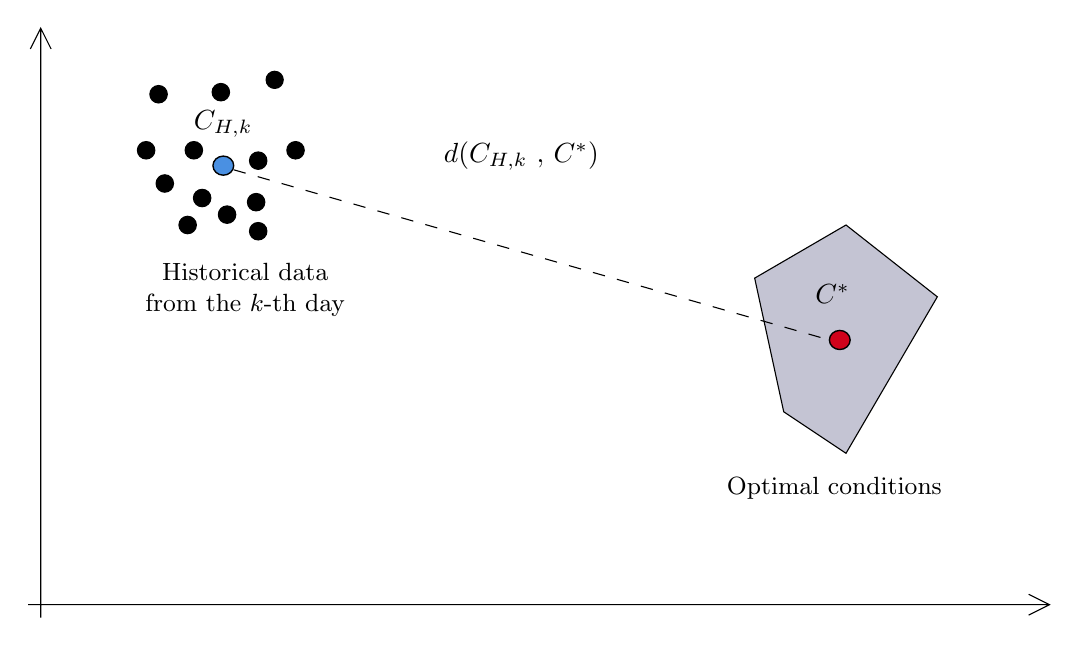
\begin{tikzpicture}[x=0.75pt,y=0.75pt,yscale=-1,xscale=1]
		%uncomment if require: \path (0,717); %set diagram left start at 0, and has height of 717
		
		%Shape: Axis 2D [id:dp4496072713140289] 
		\draw  (58,700.13) -- (550,700.13)(64.03,422.4) -- (64.03,706.4) (540,695.13) -- (550,700.13) -- (540,705.13) (59.03,432.4) -- (64.03,422.4) -- (69.03,432.4)  ;
		%Shape: Circle [id:dp06215554504361531] 
		\draw  [fill={rgb, 255:red, 0; green, 0; blue, 0 }  ,fill opacity=1 ] (133.6,481.2) .. controls (133.6,478.88) and (135.48,477) .. (137.8,477) .. controls (140.12,477) and (142,478.88) .. (142,481.2) .. controls (142,483.52) and (140.12,485.4) .. (137.8,485.4) .. controls (135.48,485.4) and (133.6,483.52) .. (133.6,481.2) -- cycle ;
		%Shape: Circle [id:dp22652234947291816] 
		\draw  [fill={rgb, 255:red, 0; green, 0; blue, 0 }  ,fill opacity=1 ] (182.6,481.2) .. controls (182.6,478.88) and (184.48,477) .. (186.8,477) .. controls (189.12,477) and (191,478.88) .. (191,481.2) .. controls (191,483.52) and (189.12,485.4) .. (186.8,485.4) .. controls (184.48,485.4) and (182.6,483.52) .. (182.6,481.2) -- cycle ;
		%Shape: Circle [id:dp7411954551562622] 
		\draw  [fill={rgb, 255:red, 0; green, 0; blue, 0 }  ,fill opacity=1 ] (172.6,447.26) .. controls (172.6,444.98) and (174.45,443.13) .. (176.74,443.13) .. controls (179.02,443.13) and (180.87,444.98) .. (180.87,447.26) .. controls (180.87,449.55) and (179.02,451.4) .. (176.74,451.4) .. controls (174.45,451.4) and (172.6,449.55) .. (172.6,447.26) -- cycle ;
		%Shape: Circle [id:dp9342194323542646] 
		\draw  [fill={rgb, 255:red, 0; green, 0; blue, 0 }  ,fill opacity=1 ] (110.6,481.2) .. controls (110.6,478.88) and (112.48,477) .. (114.8,477) .. controls (117.12,477) and (119,478.88) .. (119,481.2) .. controls (119,483.52) and (117.12,485.4) .. (114.8,485.4) .. controls (112.48,485.4) and (110.6,483.52) .. (110.6,481.2) -- cycle ;
		%Shape: Circle [id:dp7509634202671536] 
		\draw  [fill={rgb, 255:red, 0; green, 0; blue, 0 }  ,fill opacity=1 ] (130.6,517.2) .. controls (130.6,514.88) and (132.48,513) .. (134.8,513) .. controls (137.12,513) and (139,514.88) .. (139,517.2) .. controls (139,519.52) and (137.12,521.4) .. (134.8,521.4) .. controls (132.48,521.4) and (130.6,519.52) .. (130.6,517.2) -- cycle ;
		%Shape: Circle [id:dp3389656361514962] 
		\draw  [fill={rgb, 255:red, 0; green, 0; blue, 0 }  ,fill opacity=1 ] (119.6,497.2) .. controls (119.6,494.88) and (121.48,493) .. (123.8,493) .. controls (126.12,493) and (128,494.88) .. (128,497.2) .. controls (128,499.52) and (126.12,501.4) .. (123.8,501.4) .. controls (121.48,501.4) and (119.6,499.52) .. (119.6,497.2) -- cycle ;
		%Shape: Circle [id:dp7223141295117336] 
		\draw  [fill={rgb, 255:red, 0; green, 0; blue, 0 }  ,fill opacity=1 ] (149.6,512.2) .. controls (149.6,509.88) and (151.48,508) .. (153.8,508) .. controls (156.12,508) and (158,509.88) .. (158,512.2) .. controls (158,514.52) and (156.12,516.4) .. (153.8,516.4) .. controls (151.48,516.4) and (149.6,514.52) .. (149.6,512.2) -- cycle ;
		%Shape: Circle [id:dp7582728872550809] 
		\draw  [fill={rgb, 255:red, 0; green, 0; blue, 0 }  ,fill opacity=1 ] (116.6,454.2) .. controls (116.6,451.88) and (118.48,450) .. (120.8,450) .. controls (123.12,450) and (125,451.88) .. (125,454.2) .. controls (125,456.52) and (123.12,458.4) .. (120.8,458.4) .. controls (118.48,458.4) and (116.6,456.52) .. (116.6,454.2) -- cycle ;
		%Shape: Circle [id:dp49904732080555536] 
		\draw  [fill={rgb, 255:red, 0; green, 0; blue, 0 }  ,fill opacity=1 ] (163.6,506.2) .. controls (163.6,503.88) and (165.48,502) .. (167.8,502) .. controls (170.12,502) and (172,503.88) .. (172,506.2) .. controls (172,508.52) and (170.12,510.4) .. (167.8,510.4) .. controls (165.48,510.4) and (163.6,508.52) .. (163.6,506.2) -- cycle ;
		%Shape: Circle [id:dp9713308312029804] 
		\draw  [fill={rgb, 255:red, 0; green, 0; blue, 0 }  ,fill opacity=1 ] (164.6,486.2) .. controls (164.6,483.88) and (166.48,482) .. (168.8,482) .. controls (171.12,482) and (173,483.88) .. (173,486.2) .. controls (173,488.52) and (171.12,490.4) .. (168.8,490.4) .. controls (166.48,490.4) and (164.6,488.52) .. (164.6,486.2) -- cycle ;
		%Shape: Circle [id:dp6213316985023771] 
		\draw  [fill={rgb, 255:red, 0; green, 0; blue, 0 }  ,fill opacity=1 ] (164.6,520.2) .. controls (164.6,517.88) and (166.48,516) .. (168.8,516) .. controls (171.12,516) and (173,517.88) .. (173,520.2) .. controls (173,522.52) and (171.12,524.4) .. (168.8,524.4) .. controls (166.48,524.4) and (164.6,522.52) .. (164.6,520.2) -- cycle ;
		%Shape: Polygon [id:ds0377823447882647] 
		\draw [fill={rgb, 255:red, 20; green, 20; blue, 80 }  ,fill opacity=0.25 ] (452,517.2) -- (496,551.8) -- (452,627.2) -- (422,607.2) -- (408,542.8) -- cycle ;
		%Flowchart: Summing Junction [id:dp4210872697663528] 
		\draw  [fill={rgb, 255:red, 74; green, 144; blue, 226 }  ,fill opacity=1 ][line width=0.5]  (147,488.6) .. controls (147,486.06) and (149.24,484) .. (152,484) .. controls (154.76,484) and (157,486.06) .. (157,488.6) .. controls (157,491.14) and (154.76,493.2) .. (152,493.2) .. controls (149.24,493.2) and (147,491.14) .. (147,488.6) -- cycle ;% \draw  [line width=1.5]  (148.46,485.35) -- (155.54,491.85) ; \draw  [line width=1.5]  (155.54,485.35) -- (148.46,491.85) ;
		%Shape: Circle [id:dp3856640767966395] 
		\draw  [fill={rgb, 255:red, 0; green, 0; blue, 0 }  ,fill opacity=1 ] (137.6,504.2) .. controls (137.6,501.88) and (139.48,500) .. (141.8,500) .. controls (144.12,500) and (146,501.88) .. (146,504.2) .. controls (146,506.52) and (144.12,508.4) .. (141.8,508.4) .. controls (139.48,508.4) and (137.6,506.52) .. (137.6,504.2) -- cycle ;
		%Flowchart: Summing Junction [id:dp21052777836013448] 
		\draw  [fill={rgb, 255:red, 208; green, 2; blue, 27 }  ,fill opacity=1 ][line width=0.5]  (444,572.6) .. controls (444,570.06) and (446.24,568) .. (449,568) .. controls (451.76,568) and (454,570.06) .. (454,572.6) .. controls (454,575.14) and (451.76,577.2) .. (449,577.2) .. controls (446.24,577.2) and (444,575.14) .. (444,572.6) -- cycle ; %\draw  [line width=1.5]  (445.46,569.35) -- (452.54,575.85) ; \draw  [line width=1.5]  (452.54,569.35) -- (445.46,575.85) ;
		%Straight Lines [id:da05984024528227749] 
		\draw  [dash pattern={on 4.5pt off 4.5pt}]  (157,490.6) -- (444,572.6) ;
		%Shape: Circle [id:dp618933165821857] 
		\draw  [fill={rgb, 255:red, 0; green, 0; blue, 0 }  ,fill opacity=1 ] (146.6,453.2) .. controls (146.6,450.88) and (148.48,449) .. (150.8,449) .. controls (153.12,449) and (155,450.88) .. (155,453.2) .. controls (155,455.52) and (153.12,457.4) .. (150.8,457.4) .. controls (148.48,457.4) and (146.6,455.52) .. (146.6,453.2) -- cycle ;
		
		% Text Node
		\draw (104,534.4) node [anchor=north west][inner sep=0.75pt]  [font=\small] [align=left] {\begin{minipage}[lt]{85.87pt}\setlength\topsep{0pt}
				\begin{center}
					Historical data\\from the $k$-th day
				\end{center}
				
		\end{minipage}};
		% Text Node
		\draw (393,637.4) node [anchor=north west][inner sep=0.75pt]  [font=\small] [align=left] {\begin{minipage}[lt]{78.21pt}\setlength\topsep{0pt}
				\begin{center}
					Optimal conditions
				\end{center}
				
		\end{minipage}};
		% Text Node
		\draw (136.6,460.6) node [anchor=north west][inner sep=0.75pt]    {$C_{H,k}$};
		% Text Node
		\draw (436,544.4) node [anchor=north west][inner sep=0.75pt]    {$C^*$};
		% Text Node
		\draw (257,475.8) node [anchor=north west][inner sep=0.75pt]    {$d( C_{H,k} \ \mathbf{,}\ C^*)$};
		% Text Node
		%\draw (100,362.8) node [anchor=north west][inner sep=0.75pt]    {$P( X_{t+1} =D_{k+1} \mid X_{t} =D_{k}) \coloneq \ 1-\frac{\displaystyle d( C_{H,k} \ ,\ C_{O})}{\displaystyle\max_{l\in \{1,2,\dots, 365\}} \ \{d( C_{H,l} \ ,\ C_{O})\}} \ =\ \lambda _{k}.$};
	\end{tikzpicture}
	\caption{Distancia entre las condiciones agroclimáticas para el desarrollo óptimo del maíz y las condiciones agroclimáticas históricamente reportadas para el $k$-ésimo día del año. Los círculos en color negro representan los datos agroclimáticos reportados anualmente para el $k$-ésimo día del año mientras que el polígono sombreado en color gris representa la región de parámetros agroclimáticos, ideales para el desarrollo del maíz. Los círculos de color azul y rojo indican los centroides de los datos históricos ($C_{H,k}$) y la región óptima ($C^*$), respectivamente. Por último, $d(\cdot\mathbf{,} \cdot)$ denota una distancia por definir; por ejemplo, la distancia Euclidiana o la distancia Manhattan.}
	\label{Distance}
\end{figure}

Para ilustrar lo discutido en la Ecuación \eqref{TransitionProbs}, se tiene la matriz estocástica $A\in \mathcal{M}_{366\times366}(\R)$, ver Ecuación \eqref{StochasticMatrix}. Asimismo se construyó un diagrama de transición
en donde se muestra tanto la estructura cíclica como proceso estocástico que subyacen en la modelación del problema, ver Fig. \ref{Transicion}.


\begin{equation}
	A=  \begin{bNiceMatrix}[%
		first-row, 
		first-col]
		& D_1 & D_2 &D_3& D_4&\cdots &D_{364}&D_{365}&F \\
		D_1 & 0 & \lambda_1  &0  &0 & \cdots &0& 0 & 1-\lambda_1\\
		D_2 & 0 & 0  &\lambda_2  &0 & \cdots &0& 0 & 1-\lambda_2\\
		&&&&&&&\\
		\vdots\phantom{d} &&&&&\ddots&&&\vdots\\
		&&&&&&&\\
		D_{364} & 0 & 0  &0 &0 & \cdots &0& \lambda_{364}  & 1-\lambda_{364}\\
		D_{365} & \lambda_{365}   & 0  &0 &0 & \cdots &0& 0 & 1-\lambda_{365}\\
		F& 0  & 0  &0 &0 & \cdots &0& 0 & 1
	\end{bNiceMatrix}.
	\label{StochasticMatrix}
\end{equation}

\begin{figure}[ht]
	\centering
	\shorthandoff{<>}
	\resizebox{0.6\textwidth}{!}{
		\begin{tikzpicture}[
			>=Stealth,
			state/.style={draw, circle, minimum size=14mm, line width=0.8pt},
			invisible/.style={circle, minimum size=14mm, draw=none},
			arrow/.style={->, line width=0.8pt}
			]
			
			% Centro
			\node[state] (F) at (0,0) {$F$};
			
			% Hexágono
			\node[state] (D1)   at (180:3.2cm) {$D_{1}$};
			\node[state] (D2)   at (240:3.2cm) {$D_{2}$};
			\node[invisible] (dots1) at (300:3.2cm) {};
			\node[state] (Di)   at (0:3.2cm) {$D_{i}$};
			\node[invisible] (dots2) at (60:3.2cm) {};
			\node[state] (D365) at (120:3.2cm) {$D_{365}$};
			
			% Ciclo
			\path[arrow]
			(D1) edge[bend right=15] 
			node[pos=0.3, sloped, below] {$\lambda_{1}$} (D2)
			
			(D2) edge[bend right=15] 
			node[pos=0.5, sloped, below] {$\lambda_{2}$} (dots1)
			
			(dots1) edge[bend right=15]
			node[pos=0.5, sloped, below] {$\lambda_{i-1}$} (Di)
			
			(Di) edge[bend right=15] 
			node[pos=0.4, sloped, above] {$\lambda_{i}$} (dots2)
			
			(dots2) edge[bend right=15]
			node[pos=0.5, sloped, above] {$\lambda_{364}$} (D365)
			
			(D365) edge[bend right=15] 
			node[pos=0.5, sloped, above] {$\lambda_{365}$} (D1);
			
			% Hacia F
			\path[arrow]
			(D1) edge node[pos=0.55,above] {$1-\lambda_{1}$} (F)
			(D2) edge node[pos=0.55, sloped, above] {$1-\lambda_{2}$} (F)
			(Di) edge node[pos=0.55, above] {$1-\lambda_{i}$} (F)
			(D365) edge node[pos=0.55, sloped, above] {$1-\lambda_{365}$} (F);
			
			% Loop
			\path[arrow]
			(F) edge[
			loop,
			out=320, 
			in=300,
			looseness=8
			] node[pos=0.8, xshift=10pt, yshift=-10pt] {$1$} (F);
			
			% Puntos suspensivos
			\node[font=\large, rotate=35] at (300:3.1cm) {$\cdots$};
			\node[font=\large, rotate=-30] at (60:3.1cm) {$\cdots$};
			
		\end{tikzpicture}
	}
	\shorthandon{<>}
	\caption{Diagrama de transición diaria de la factibilidad de siembra. El estado $F$ indica el fracaso del proceso de siembra, mientras que los estados $D_i$, $i\in\{1,2,\ldots,365\}$, denotan el $i$-ésimo día del año calendario. 
		Cuando el proceso $X$ se encuentra en un estado $D_i$, se interpreta que, en dicho día, la semilla continúa su desarrollo de manera adecuada, es decir, que el proceso no ha sido absorbido por el estado $F$ como consecuencia de las condiciones agroambientales del entorno. Para cada $i$, $\lambda_i$ denota la probabilidad de transición de $D_i$ a $D_{i+1}$, y $1-\lambda_i$ la probabilidad de transición de $D_i$ a $F$.}
	\label{Transicion}
\end{figure}


As in the work of \cite{Waha_2011}, for model simplicity, we have assumed that crop-specific thresholds are applicable globally.
$$\mathcal{C}^*= (11.10, 75,9,75)$$
